\documentclass[draft]{spieman}

\usepackage[utf8]{inputenc} \usepackage{amsmath,amsfonts,amssymb}
\usepackage{graphicx} \usepackage{grffile} \usepackage[colorlinks=true,
allcolors=blue]{hyperref} \usepackage{pdflscape} \usepackage{afterpage}

% Title definition
\title {The WIYN One Degree Imager in 2018: An Extended 30-Detector Focal Plane
and Operational Challenges}

\author[a,b]{Daniel R. Harbeck} \author[c]{Mike Lesser} \author[b]{Wilson Liu}
\author[d]{Bob Stupak} \author[d]{Ron George} \author[d]{Ron Harris}
\author[d]{Gary Poczulp} \author[d]{Jayadev Rajagopal} \author[e]{Ralf Kotulla}
\author[c]{David Ouellete} \author[e]{Eric Hooper} \author[e]{Michael Smith}
\author[e]{Dustin Mason} \author[f]{Peter Onaka} \author[f]{Greg Chin}
\author[d]{Emily Hunting} \author[d]{Robert Christensen}

\affil[a]{Las Cumbres Observatory, Goleta, CA (USA)} \affil[b]{WIYN Observatory,
Tucson, AZ (USA)} \affil[c]{The University of Arizona, Tucson, AZ (USA)}
\affil[d]{NOAO, Tucson, AZ (USA)} \affil[e]{University of Wisconsin, Madison, WI
(USA)} \affil[f]{University of Hawaii, Honolulu, HI (USA)}

\newcommand{\electron}{e$^-$\xspace} \newcommand{\degree}{$^\circ$\xspace}


\begin{document}

\maketitle

\begin{abstract}
    
We report on the performance of the upgraded One Degree Imager (ODI) at the WIYN
3.5 meter telescope at the Kitt Peak Observatory. The focal plane has been
expanded by additional sixteen detectors in spring / summer 2015. The now thirty
Orthogonal Transfer Array CCD detectors has a field of view of 40’ x 48’ on the
sky. The newly added detectors underwent a design revision to mitigate reduced
charge transfer efficiency under low light conditions (fat zero problem). We
discuss the imaging performance and challenges in the photometric calibration of
the wide field of view, helped by the addition of telescope baffles. In a
parallel project, we upgraded the instrument's filter mechanism, where a
degrading worm-gear mechanism was replaced by a chain drive that is operating
faster and at a higher reliability level. Two more filters, a U band and narrow
band filter were added to the instrument's complement. We will review the
lessons learned during nearly three years of operating the instrument in the
observatory environment and discuss infrastructure upgrades that were driven by
ODI's needs. 

\end{abstract}


%>>>> Include a list of keywords after the abstract

\keywords{Ground based instrumentation, wide field imaging, CCD, Orthogonal
    Transfer Array, Observatory Operations}

%%%%%%%%%%%%%%%%%%%%%%%%%%%%%%%%%%%%%%%%%%%%%%%%%%%%%%%%%%%%%
\section{Introduction}

The One Degree Imager (ODI) has been the major instrument development project
from 2004 to 2016 for the WIYN 3.5 meter telescope (Kitt Peak, Arizona), and its
design has been documented in various SPIE conference contributions
\cite{jacoby2002,Harbeck2008,Jacoby2008,Yeatts2008,Harbeck2010,Yeatts2010,harbeck2014,gopu2014,}.
 The instrument is designed for a one degree  square field of view with 64 Orthogonal Transfer Array 
(OTA) CCD sensor. A first incarnation of ODI was deployed in the summer of 2012 with a partially 
populated focal plane (with 13 out of 64 detectors installed); this  incarnation of ODI was called pODI 
and was described in detail the SPIE Astronomical Telescopes + Instrumentation conference in 
2014\cite{harbeck2014}. In that paper we outlined an incremental upgrade path for the instrument to a
larger focal plane, and in 2015 we have deployed ODI with an enlarged 5x6
detector array by adding 17 new detectors; this incarnation of ODI is generally
referred to "5x6 ODI" or simply ODI, as now additional development of the focal
plane is anticipated at this time.


\section{Upgrade of the Instrument}
* Upgraded in Tucson, AZ
* 12 wafer run of Lot 7 detecors, which are a modified design to resolve a low light level charge transfer 
efficiency issue\cite{harbeck2014}. The processing and packaging of the detectors at Imaging 
Techonolgy Laboratory  (ITL, Tucson, AZ) \cite{lesser2012} yielded in 17 useful devices. The existing 13 
Lot 6 devices from the pODi focal plane and the new detectors of Lot 7 were installed into the focal 
plane  by ITL. Subsequently, the focal plane was installed back in to the dewar. 

The cryostat was refurbished during the focal plane upgrade. For once, numerous small leaks had 
developed at on ehalf of the flex circuit vacuum feed throughs. Those had been sealed by adding 
additional epoxy. 

Inside the dewar we found indication of condensed outgassing, and the dewar was thouroughly 
cleaned. 

At the time of the refurbishment, the molecular sieve material in the dewar (Zeolite 5-A) had lost its 
ability to adsorb gas in the dewar, leading to unmanageable short vacuum hold time of a few days only; 
it is  suspected 
that it was saturated by water, and it was hence replaced with fresh material. Nevertheless, about a 
year after the upgrade we found the getter material to have saturated again, and at that time it was 
replaced with a hydrophobic Zeolite ZSM-5. we found that this getter material performs equally well as 
the fresh Zeolite 5-A, and after over two years in operations, there is no indication of saturation. 


\subsection{Focal Plane  Performance}

As already demonstrated, the lowlight level charge transfer efficiency under low light level. Since the 
5x6ODI focal plane also utilizes  Lot 6 detectors with the known issue, observations that depend on 
the ful lfield of view still require minimum exposure level of the order of 100 electrons.
 The amplifier glow observerd in Lot 6 detectors is largely unchanged for Lot 6. The amplifier glow is 
 mitigated by shutting down the output drain for all detectors but those that are required for guide star 
 acquisition. 


Controlling the output drain for the detectors leads to a change in the dissipated power per detector. 
For pODI we estimated that the difference between output drain on and off amounts ot the order of 
0.5W power difference per detector. Given 30 there are now detectors in the focal plane, during the 
readout time while OD is turned on (typically 6.5 seconds) there will be an additional 30 Watts 
dissipated in the focal plane. This can caus temeperature variations in the focal plane of the order of 
several  few tens of  degree K, in particular during a high cadence use case. While the total cooling 
power of the ODI focal plane would have been sufficient to cool the detectors, the temperature would 
not be stable enough in a fully populated focal plane that would require varying the output drain 
voltage. 


The Stargrasp CD controller used in ODI can control one or two detectors. For pODI, a maximum of one 
detector was connected per CCD , 1/3 of the detectors remain on one to one connections.  For 
crosstalk performance between detectors connected to the same controller was untested before the 
upgrade, and after the upgrade we found no evidence af ony additional crosstalk. As before crosstalk 
exists only between the amplifier of a single OTA device. 



\subsection{Tuning the acquisition software}

The ODI data acquisition is described in detail in previous SPIE
 contributions\cite{Yeatts2008,Yeatts2010}.
In short, the focal plane is read out by 20 Stargrasp CCD controllers which
interface to a network switch via 20 separate 1GB ethernet over fiber
connections. The switch itself bundles the data connection into a 10GB network
backbone used by the ODI computers (three 24 core, 32GB RAM servers). The stream
from the 30 CCDS is collected by a single server / java virtual machine that is
managed by a JBOSS 5 application server. The data are stored to disk.

The amount of data has more than doubled (from 13 detectors to now 30), and as
the detectors are read out in parallel, so has the data rate. The scalability of
the data acquisition system was tested before the upgrade by creating a mock-up
focal plane  configuration to simulate the enlarged focal plane. This test
revealed some bottlenecks: the interval between sustained bias readouts
increased from about 25 seconds to over 40 seconds. Several bottlenecks in the
data acquisition code were identified and mitigated during the upgrade project
and commissioning phase:


\begin{enumerate} 
    
\item For pODI, all data were stored to a NFS mounted Oracle storage appliance
(ZFS....), and the data time to write fits files to disk was the major factor to
slow down the data handling process. As a mitigation we equipped the acquisition
server with a Raid 5 configured local storage array, utilizing only disks with a
6G interface. The imaging data were then slowly transfered by a background
process to the storage appliance, both as a mid-term storage and to stage data
for transfer into the ODI data archive.

\item  The simultaneous receiving of the data streams from 30 detectors posed no
major challenge over the 10GB network backbone.  However, when writing the the
data to disk we realized a significant  improvement in the write speed by
limiting the number of data streams that are written in parallel to disk. As a
mitigation, the FITS file writing routine was changed into a Callable that would
be submitted to a multi-threaded Executor with 10 threads. An additional
improvement in write performance was achieved by rewriting the fits io package
to allow writing into BufferedOutputfile,

\item As part of the data storage process, a thumbnail image is generated for
each detector to help the observer to judge image quality in real time. For
pODI, the thumbnail generation was delegated to a command line utility that was
called after the images were written to disk, reading back (and decoding) the
fits file again. Also, the thumbnail generation process was unnecessarily
serialized in the data acquisition process, i.e., telescope observations would
be blocked until thumbnail images were generated.  For 5x6 ODI we have moved the
thumbnail generation into the JVM, were the data were already in memory, hence
saving I/O and CPU time for FITS decoding. Furthermore, the generation of the
thumbnails was delegated to a lower priority background threads, making the
thumbnail generation an asynchronous process.

    
\end{enumerate}

As indicated by prior testing, the existing IT infrastructure was capable of
handling the larger focal plane after some investments into faster local
storage and by serializing write processes. The key was to serialize writing
large amounts of data to a hard drive. After each readout, about 6 seconds
are spend to flush the detector to remove residual charge, the readout
overhead is now limited by the detector and telescope performance.


\section{Filter change mechanism upgrade and performance}

\subsection{Motivation for filter drive upgrade} Initial worm drive;
unlubricated due to proximity to filters. Bronze shaving that spread
throughout instrument and facility.  Need to replace worm gears on an annual
basis. Because of the gravity vector being parallel to all optical surfaces,
the shavings have been assessed as no immediate threat to the instrument
health.

The issue was discovered a few month before the planned installation of ODI,
and because of stakeholder and schedule priorities it was decided at that
time to live with the filter drive problem and deal with it later.

\subsection{Revised design and testing}

Follow up on earlier chain drive concept, feasibility of such a drive was
tested in a prototype. Build, and tested with 10000 in / out actuations.
Worm gear dismantled afterwards, and inspected for wear. There was no
indication of problems, hence decision to continue.


\subsection{Performance of revised filter drive}






\section{Scientific performance of the upgraded instrument}

The deliveed image quality over the entire field of view as verified to be homogeneous and, when 
atmospheric conditions allow, better then 0.4" in the SDSS g' band.


\subsection{Straylight mitigation by additional baffles}

Before ODI was deployed, a detailed straylight analysis (Photon Engineering)
indicated that a significant contribution of off stray light can be expected to
fall onto the ODI focal plane. The two major contributors are (i) off-axis rays
reflecting off the tertiary mirror, then the primary mirror, and then entering
the instrument and (ii) off-axis rays reflecting off the tertiary mirror,
entering the instrument. The first stray light mode had already been addressed
by installing an additional baffle at the entrance aperture of ODI. The latter
stray light path, however, had not been mitigated yet. The impact of the
straylight is clearly visible in Figure\ref{fig_straylight}, where we show the
view through the instrument at the center and corner of the field of view.


\begin{figure}[h]
	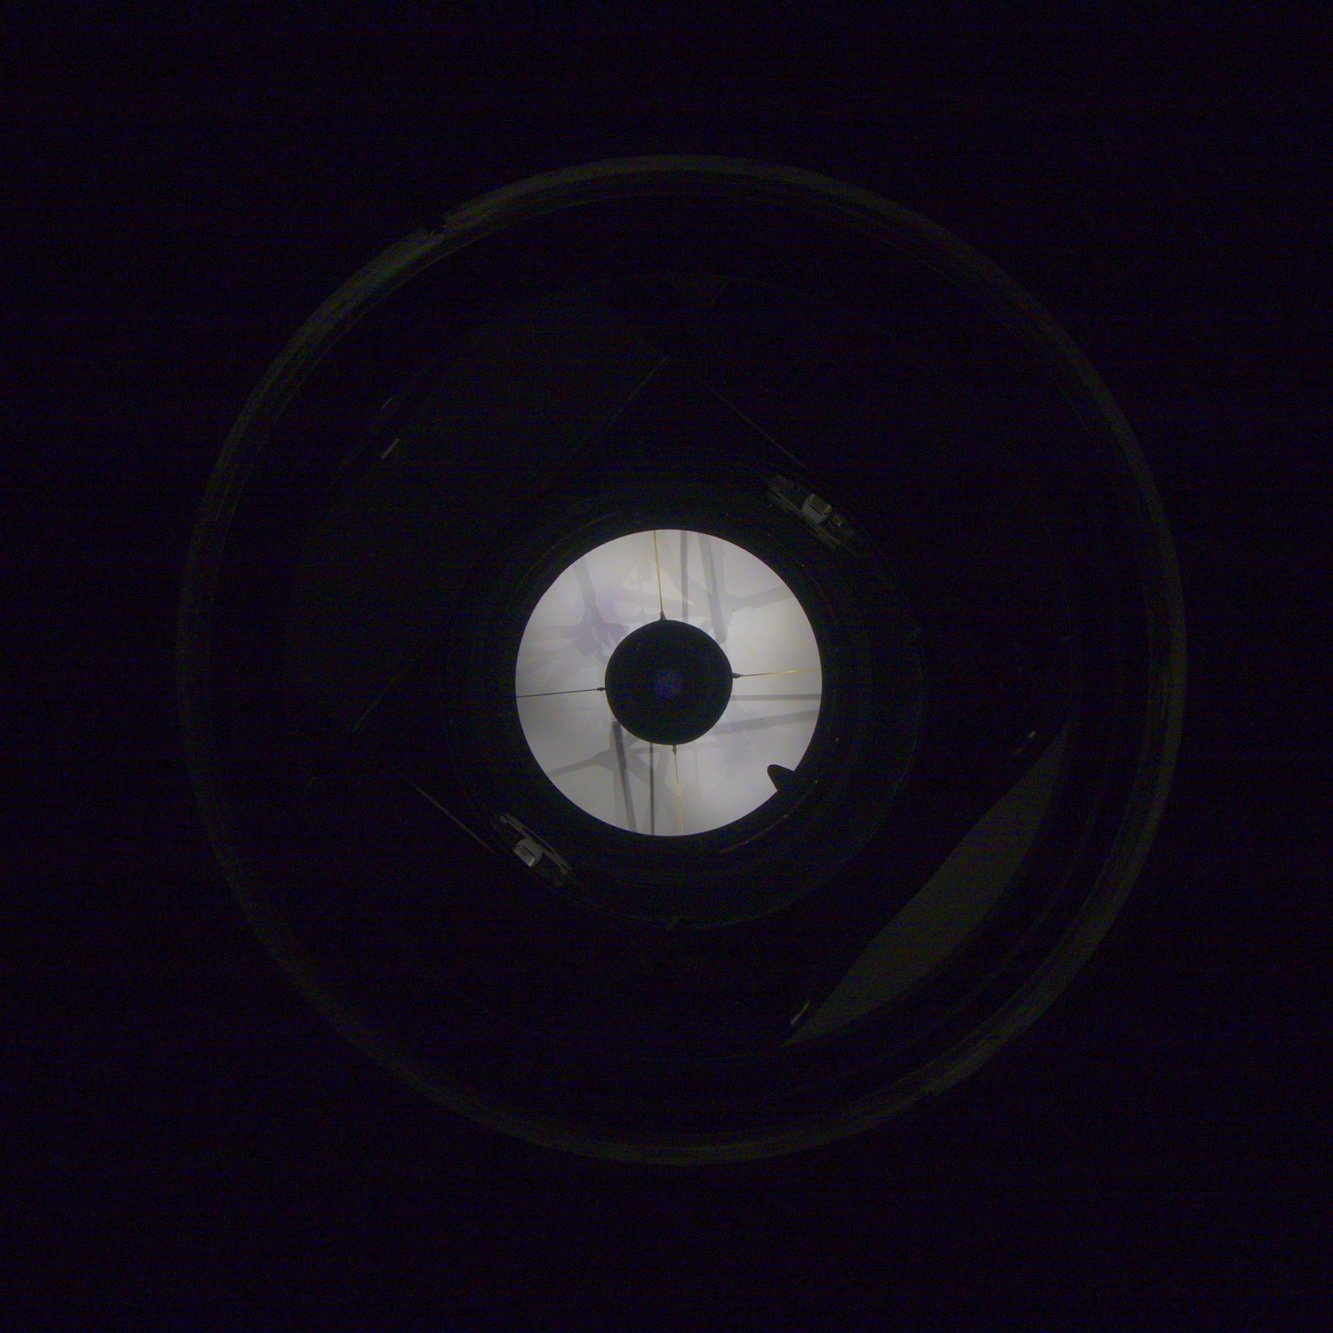
\includegraphics[width=0.49\columnwidth]{images/straylight-center.png}
	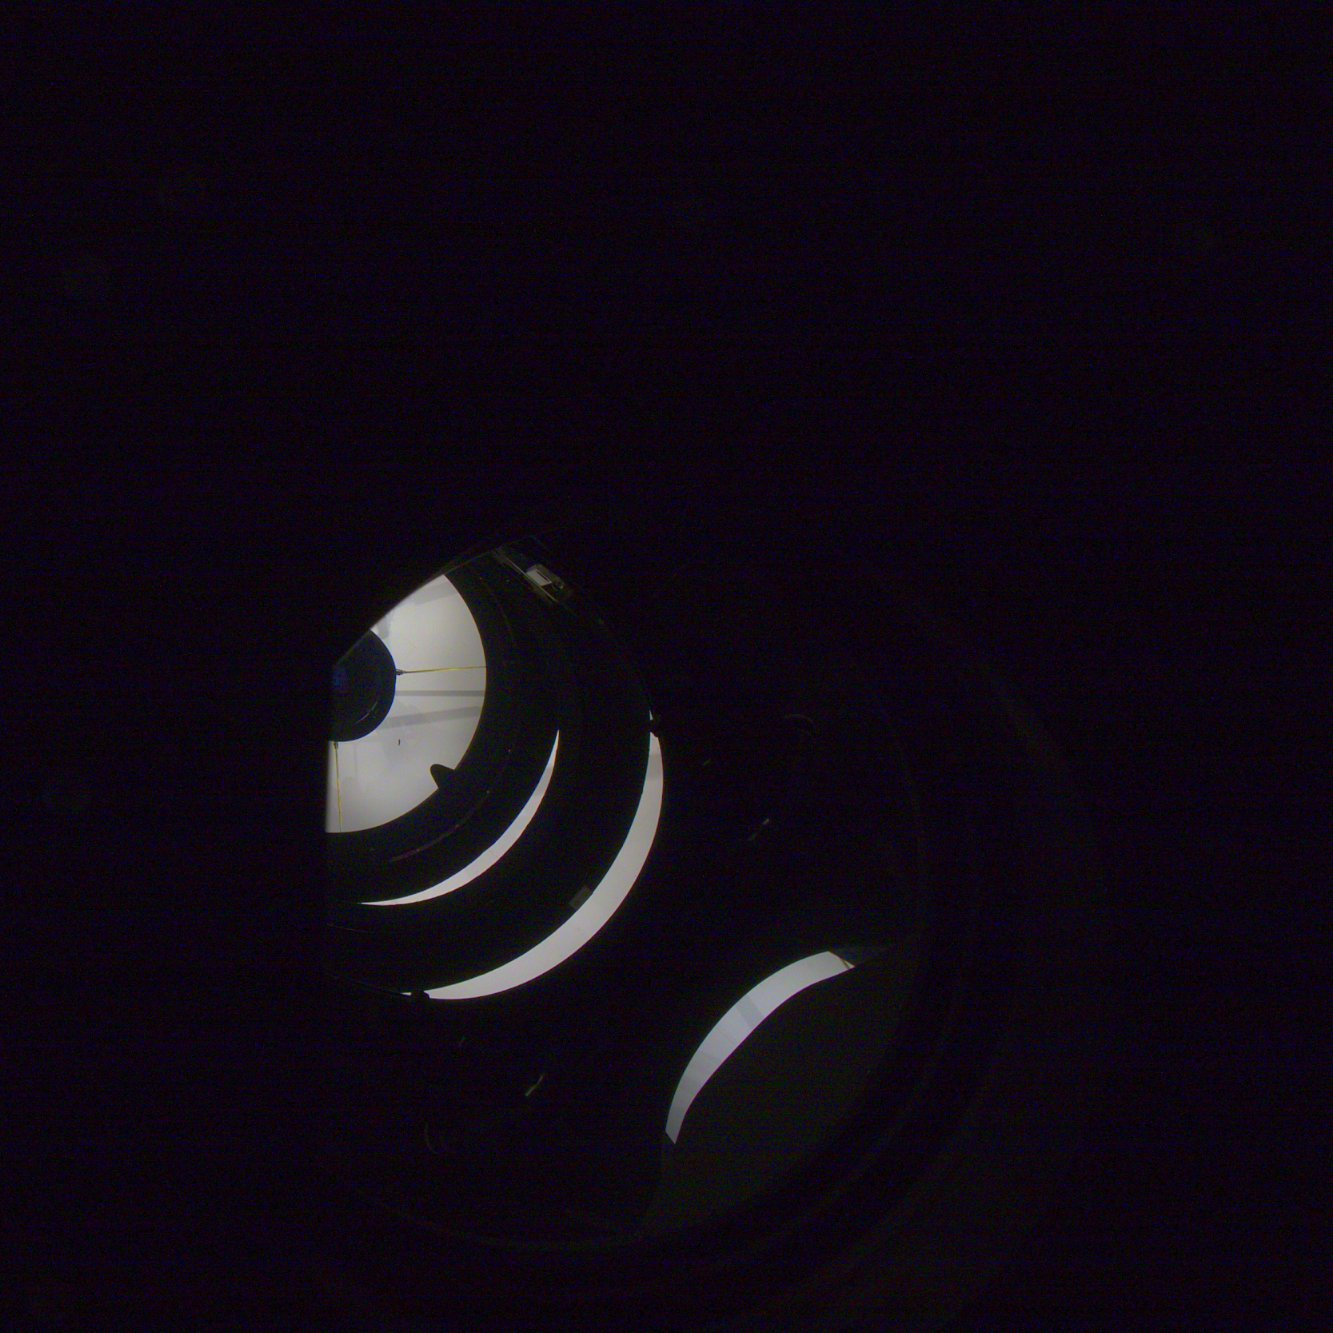
\includegraphics[width=0.49\columnwidth]{images/straylight-offcenter.png}
	\caption{\label{fig_straylight} View through the ODI instrument and telescope
		onto the WIYN flat field screen. Left: at the center of the field, where only
		the mirror pupil is a major contributor of illumination. Right: View from the
		upper left corner of the instrument. Additional stray light arcs become visible.
		the upper two arcs originate from the off-field light that enters the instrument
		directly off an reflection of the tertiary mirror. The third lower right arc is 
		due to reflection of off field light off the tertiary, onto the primary mirror,
		and  into the instrument. } 
\end{figure}


While for the initial pODI instrument with a smaller focal plane the stray
light did not significantly affect operations, the extended focal plane of
ODI was found to be indeed heavily affected by the second stray light path.
For night time observations the straylight manifests in additional
background structure, it is detrimental for the acquisition of flat field,
where the stray light contamination was determined to be of order of 30\%.

The straylight is loopsided in the instrument, i.e., looking through the
Nasmyth port, only the upper left side of port would be affected by the
stray light. The instrument rotates at the Nasmyth port, and the effect of
straylight onto flatfields can be easily demonstrated by formatting the ratio
of two flat fields with the instrument rotated by $180^\circ$ with respect
to the telescope reference frame. Figure \label{fig_flatfieldbaffle}

\afterpage{%
    \clearpage% Flush earlier floats (otherwise order might not be correct)
    \thispagestyle{empty}% empty page style (?)
    \begin{landscape}% Landscape page
        \centering % Center table
        \begin{figure} \begin{tabular}{ccccc} odi u' & odi g' & odi r & odi
                i & odi z \\ \hline \multicolumn{5}{c}{ratio of $\pm 90 \deg$ flat
                    fields, no baffle} \\ \hline
                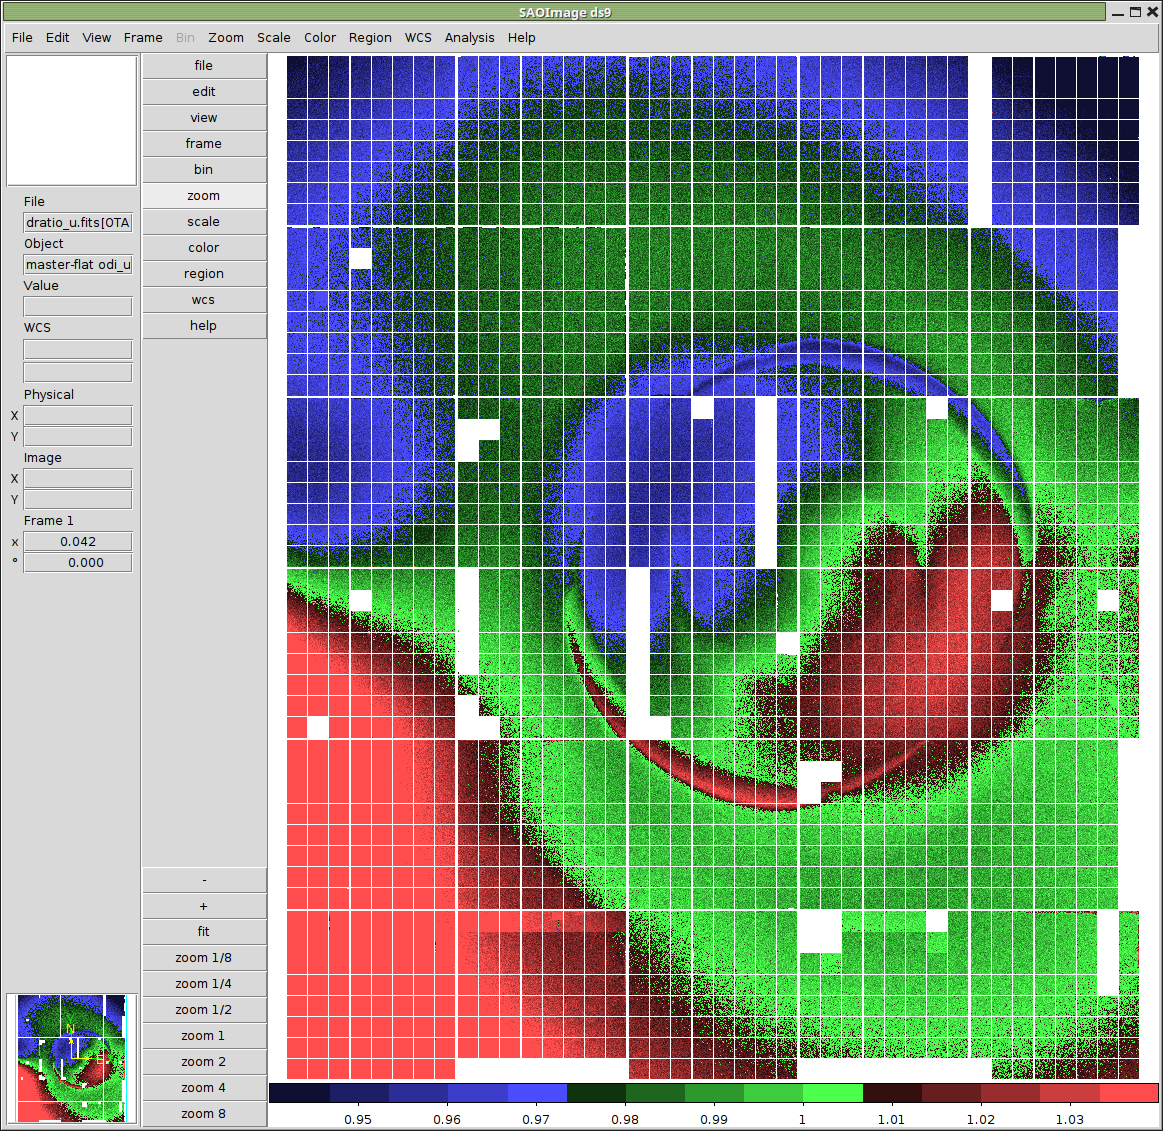
\includegraphics[width=0.2\textwidth]{images/nobaffle_u.png} &
                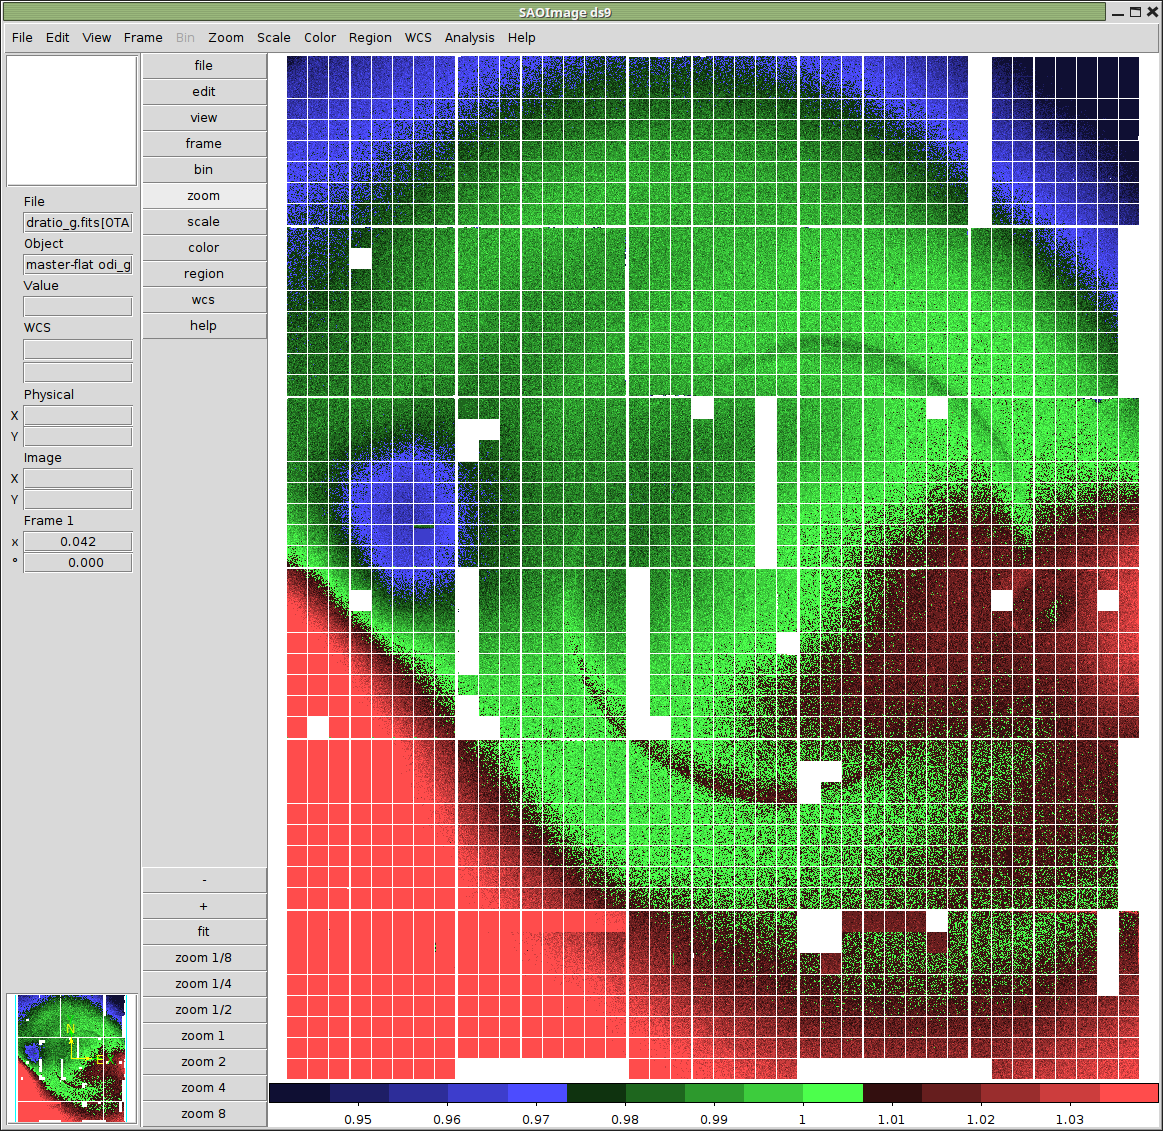
\includegraphics[width=0.2\textwidth]{images/nobaffle_g.png} &
                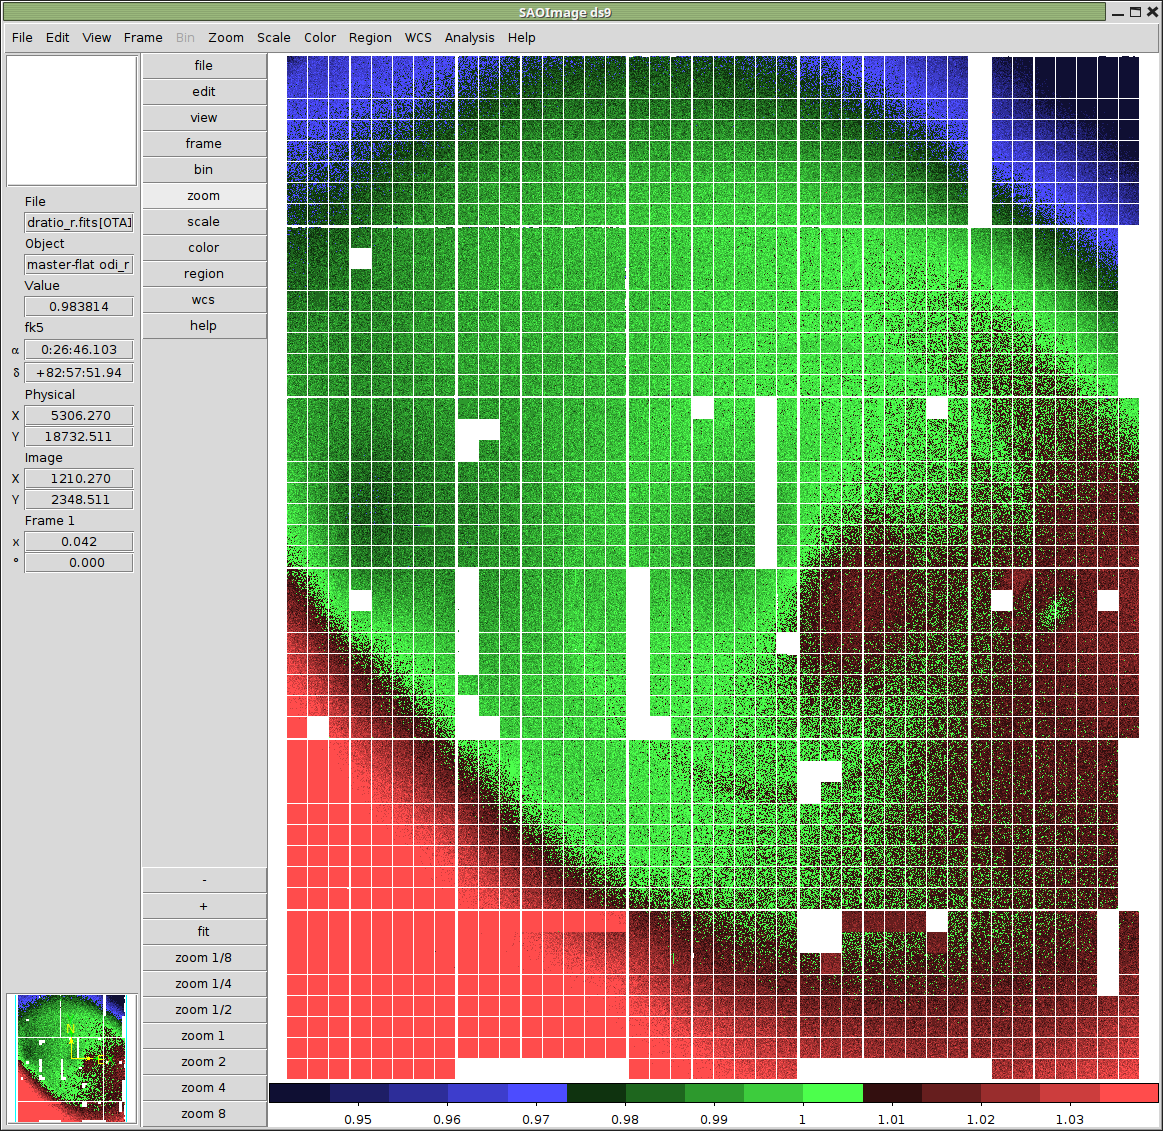
\includegraphics[width=0.2\textwidth]{images/nobaffle_r.png} &
                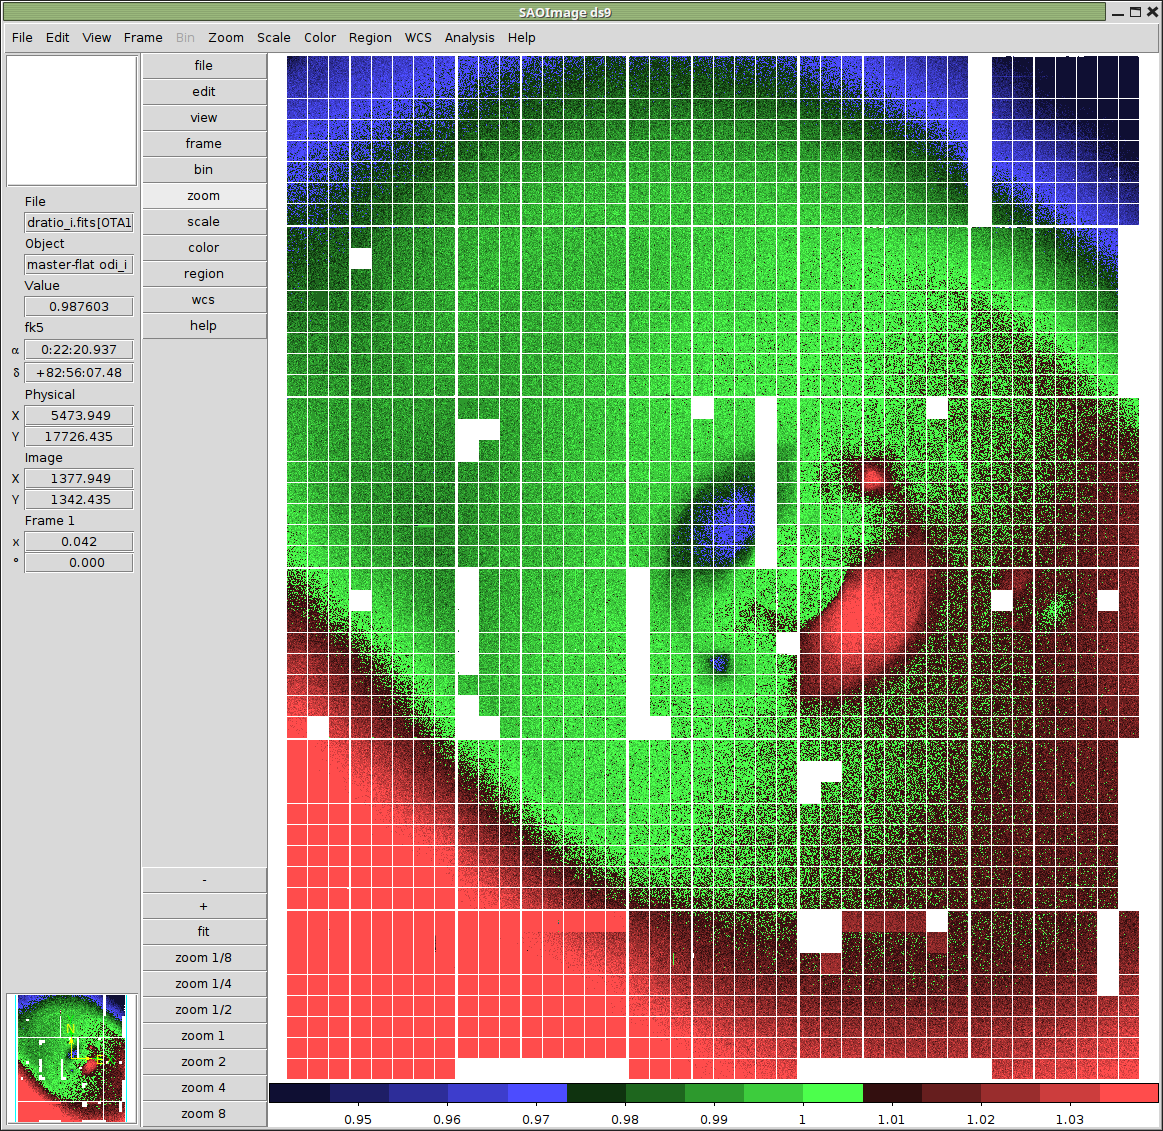
\includegraphics[width=0.2\textwidth]{images/nobaffle_i.png} &
                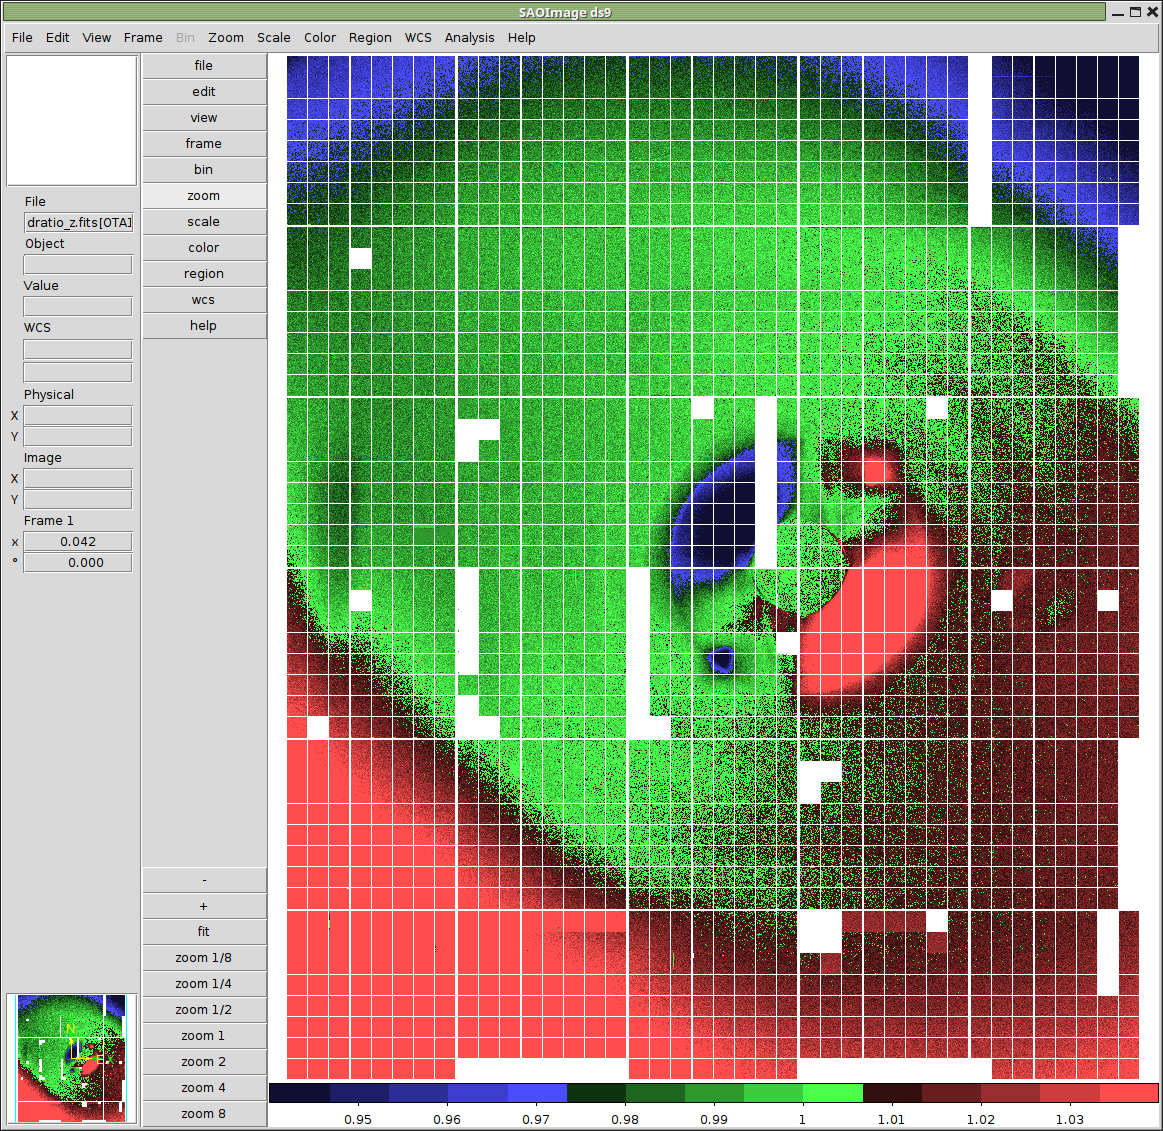
\includegraphics[width=0.2\textwidth]{images/nobaffle_z.png} \\
                \hline
                
            \end{tabular}
            
            \caption{\label{fig_flatfieldbaffle} Ratios of flat field images
                taken at an instrument rotator angle of $+90^\circ$ $-90^\circ$ 
                for all ODI broad band filters. }
            
        \end{figure}
        
    \end{landscape} 
  \clearpage% Flush page
}


\subsection{Pupil ghost suppression using a two-bladed shutter}



Reflections of the optical surfaces within WIYN One Degree Imager (ODI) produce
internal ghosting, resulting inflat fields or exposures of the night sky to form
an image of the telescope pupil. Thanks to anti-reflection coatings on the
optics, each reflection is suppressed to about about 1\%-2\% level, depending on
the actual wavelength of the light, but the residual light is still capable of
producing a significant ghosting component. ODI’s dewar window is concave, and
paired with the plane surface of the passband filter forms an imaging system
that.

\begin{figure}
	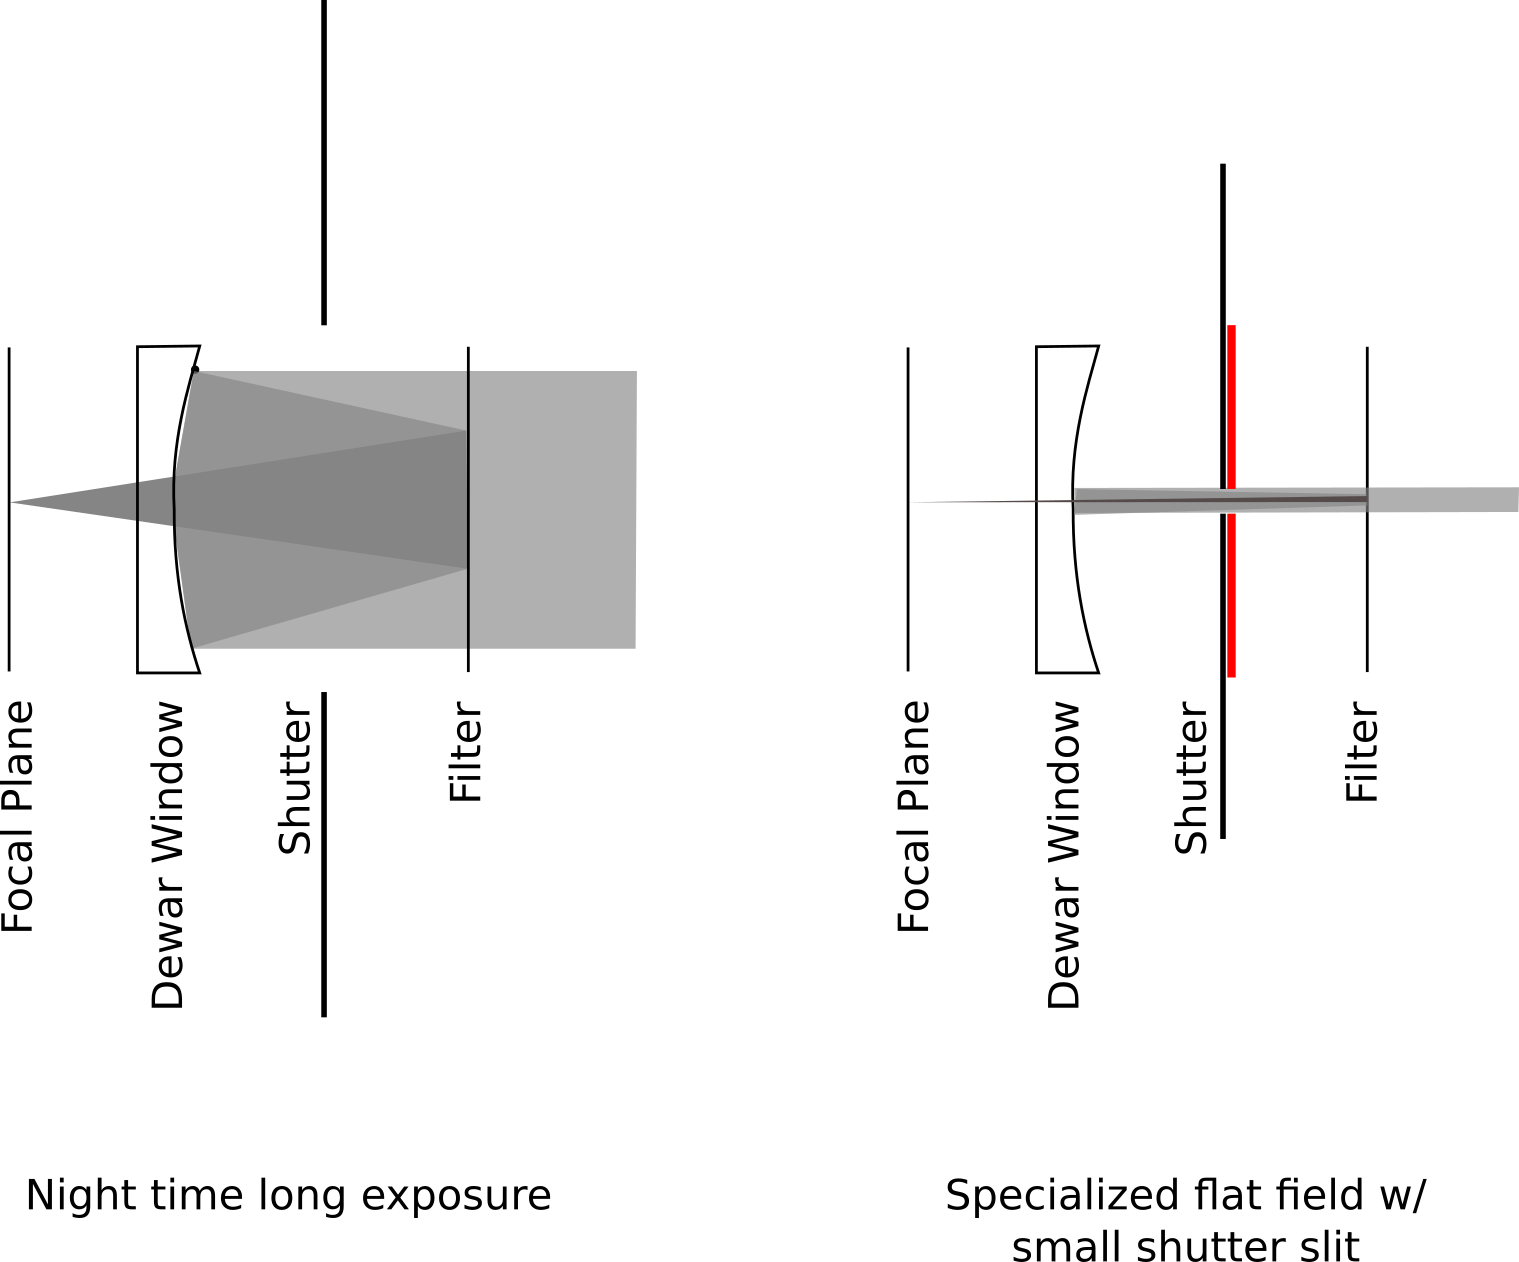
\includegraphics[height=8cm]{images/odishutterpupilghostsupression.png}
	\hspace{0.5cm} 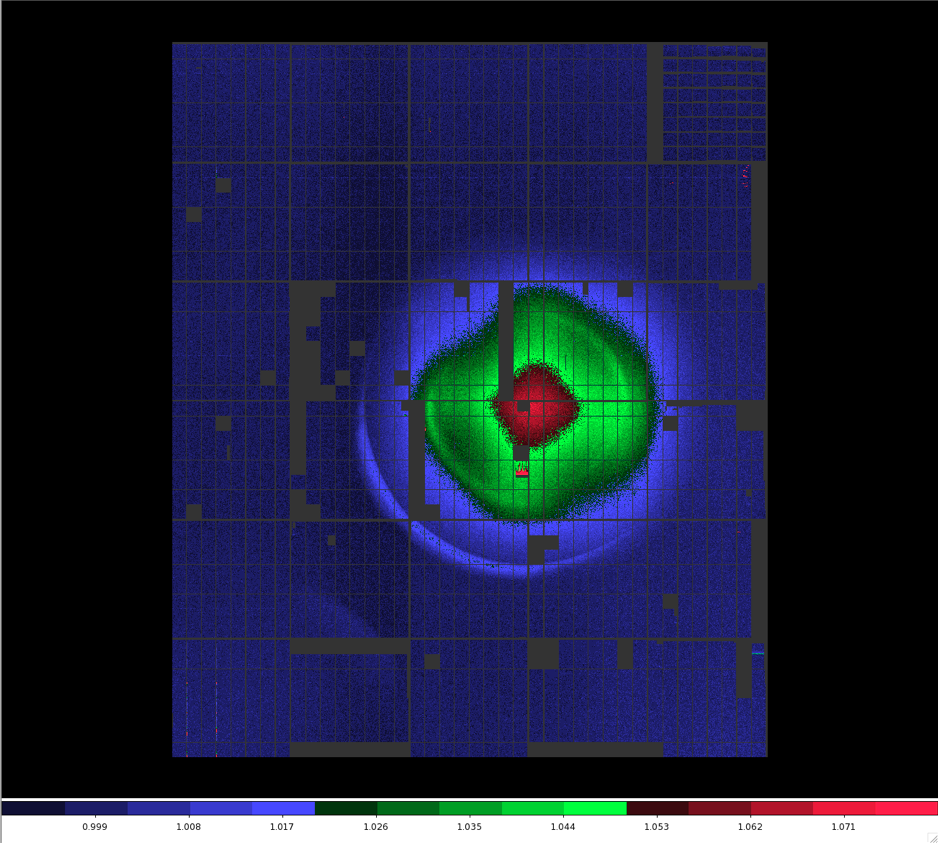
\includegraphics[height=8cm]{images/odi_layeronepg.png}
	
	\caption{ \label{fig_pupilghost}Left: Formation of the pupil ghost in ODI:  light 
		entering the instrument from the telescope (from the right) reflects of the
		concave dewar window, and the converging beam reflects of the filter to
		form an in-focus image of the telescope pupil. Right: Ratio of a flat
		field taken with different shutter modes. The sensitivity variations between
		pixels and detectors cancel out, but the excess ghosting light remains. Note
		that this ratio shows the ghosting component created by filters that are at
		a different location than in Fig. 1, and the pupil ghost is largely out of
		focus.}
	
\end{figure}

The excess light of the pupil ghost is undesirable for several reasons: In
night-sky observations it will produce an extra background component, but that
can be subtracted out. More severely, the pupil ghost also produces an extra
light component in a calibrating flat field, and if not treated, would lead to a
wrong sensitivity calibration in the affected areas.

The first method to remove the pupil ghost out of calibration images was to
model the ghost image and to then subtract it out of the flat field images. This
approach was overall successful, but is prone to adding noise and residual
errors from fitting a template to data. It remains desirable to avoid the pupil
ghost formation.

The pupil ghost was found to be greatly suppressed by the ODI shutter when the
exposure is tuned in a way where the shutter blades mostly obstruct the optical
path in front of the dewar window, and expose only via a narrow slit that moves
slowly over the focal plane. This suppression mechanism is illustrated by Figure
\ref{fig_pupilghost}. Note that, despite the shutter forming only a narrow slit,
the direct illumination of the focal plane is identical to a flat field where
the shutter completely opens.

This ghost-suppressing behavior of the shutter has been exploited already by
using very short exposure times of order of 50ms for sky flat fields, and this
new method has replaced the pupil ghost model subtraction method. However,
 this method was applicable only for situations with a very
bright flat field illumination that would support extremely short exposure
times. By lowering the travel speed of the shutter blades, however, one can
achieve the same ghost suppressing property at longer exposure times on the
focal plate. The cost, however, is that each flat field will take about 27
seconds longer, as this is the travel time of the blades (the travel time at
default speed is about 0.75 seconds).

A good demonstration of the pupil ghost suppression by the shutter is to divide
a flat field where the shutter is operated conventionally by a flat field where
the shutter was operated in the narrow-slit mode. Only the extra stray light
component should remain visible in the image, as demonstrated in Figure
\ref{fig_pupilghost}.


\subsection{Condensation}

remains issue, operational limit lowered to 70\% until full mitigation
strategy implemented.



\section{Infrastructure upgrades}

Lessons from pODI operations and early 5x6 ODI implemented:

- Helium compressors on UPS: cascade of failures: power outage leads to cooling outage leads to 
cold trap outgassing leads to vacuum interlock failure leads to warm up leads to the dark side. 

- Redundant dry air compressor and buffer tank for condensation prevention. Again. power outages 
and failures in compressor (mostly relay) had let to interruption in dry air supply.  Electronic 
data logging and alerting on dry air humidity.




\section{Summary}

With the upgrade in 2015, the ODI instrument has reached a stable state and is a scientifically useful 
instrument for the WIYN community. With the upgrade of the filter arm mechanism, the instrument 
infrastructure is robust, and only condensation of the dewar window remains a limitation for 
operations, and can be mitigated by the installation of  heater.  

It has been demonstrated before that the tip tilt image motion can be successfully compensated by 
OTA detectors.  However, the amplifier glow in ODI prohibits the use of a detector for guide star 
acquisition, and the idea of a local image motion compensation within an isokinetic patch is not 
achievable with the devices developed for ODI. But even it the amplifier glow was addressed 
successfully, 
there are practical issues with implementing a rubber focal plane as envisioned in \cite{tonry2002}: The 
density of  bright guide stars is insufficient in in some  optical passbands, in particular outside the 
galactic plane. And it is not sufficiently established how one would go about the astrometric calibration 
of a rubber focal plane.  Hence, neither the PanSTARRS survey nor the ODI instrument choose to 
operate the focal plane in the rubber mode other than for demonstration purpose.  I

ODI is now an instrument in routine operations. The choice to use  OTA detectors in ODI has largely 
complicated the operation of the focal plane and the subsequent data calibration without providing any 
benefits over a conventional CDD. If the WIYN community were to refurbish the ODI instrument it would 
be prudent to avoid OTA detectors in the future. 
 
%%%% References %%%%%
\bibliography{odi} 
\bibliographystyle{spiejour}

\end{document}
